\chapter{Results}

\section{Employing Proposed Pipeline}\label{section:employing-proposed-pipeline}

\section{Analyzing Behavioral Repertoire}\label{section:analyzing-behavioral-repertoire}

\begin{figure}[ht!]
	\centering
	\begin{subfigure}[ht!]{0.85\linewidth}
		\centering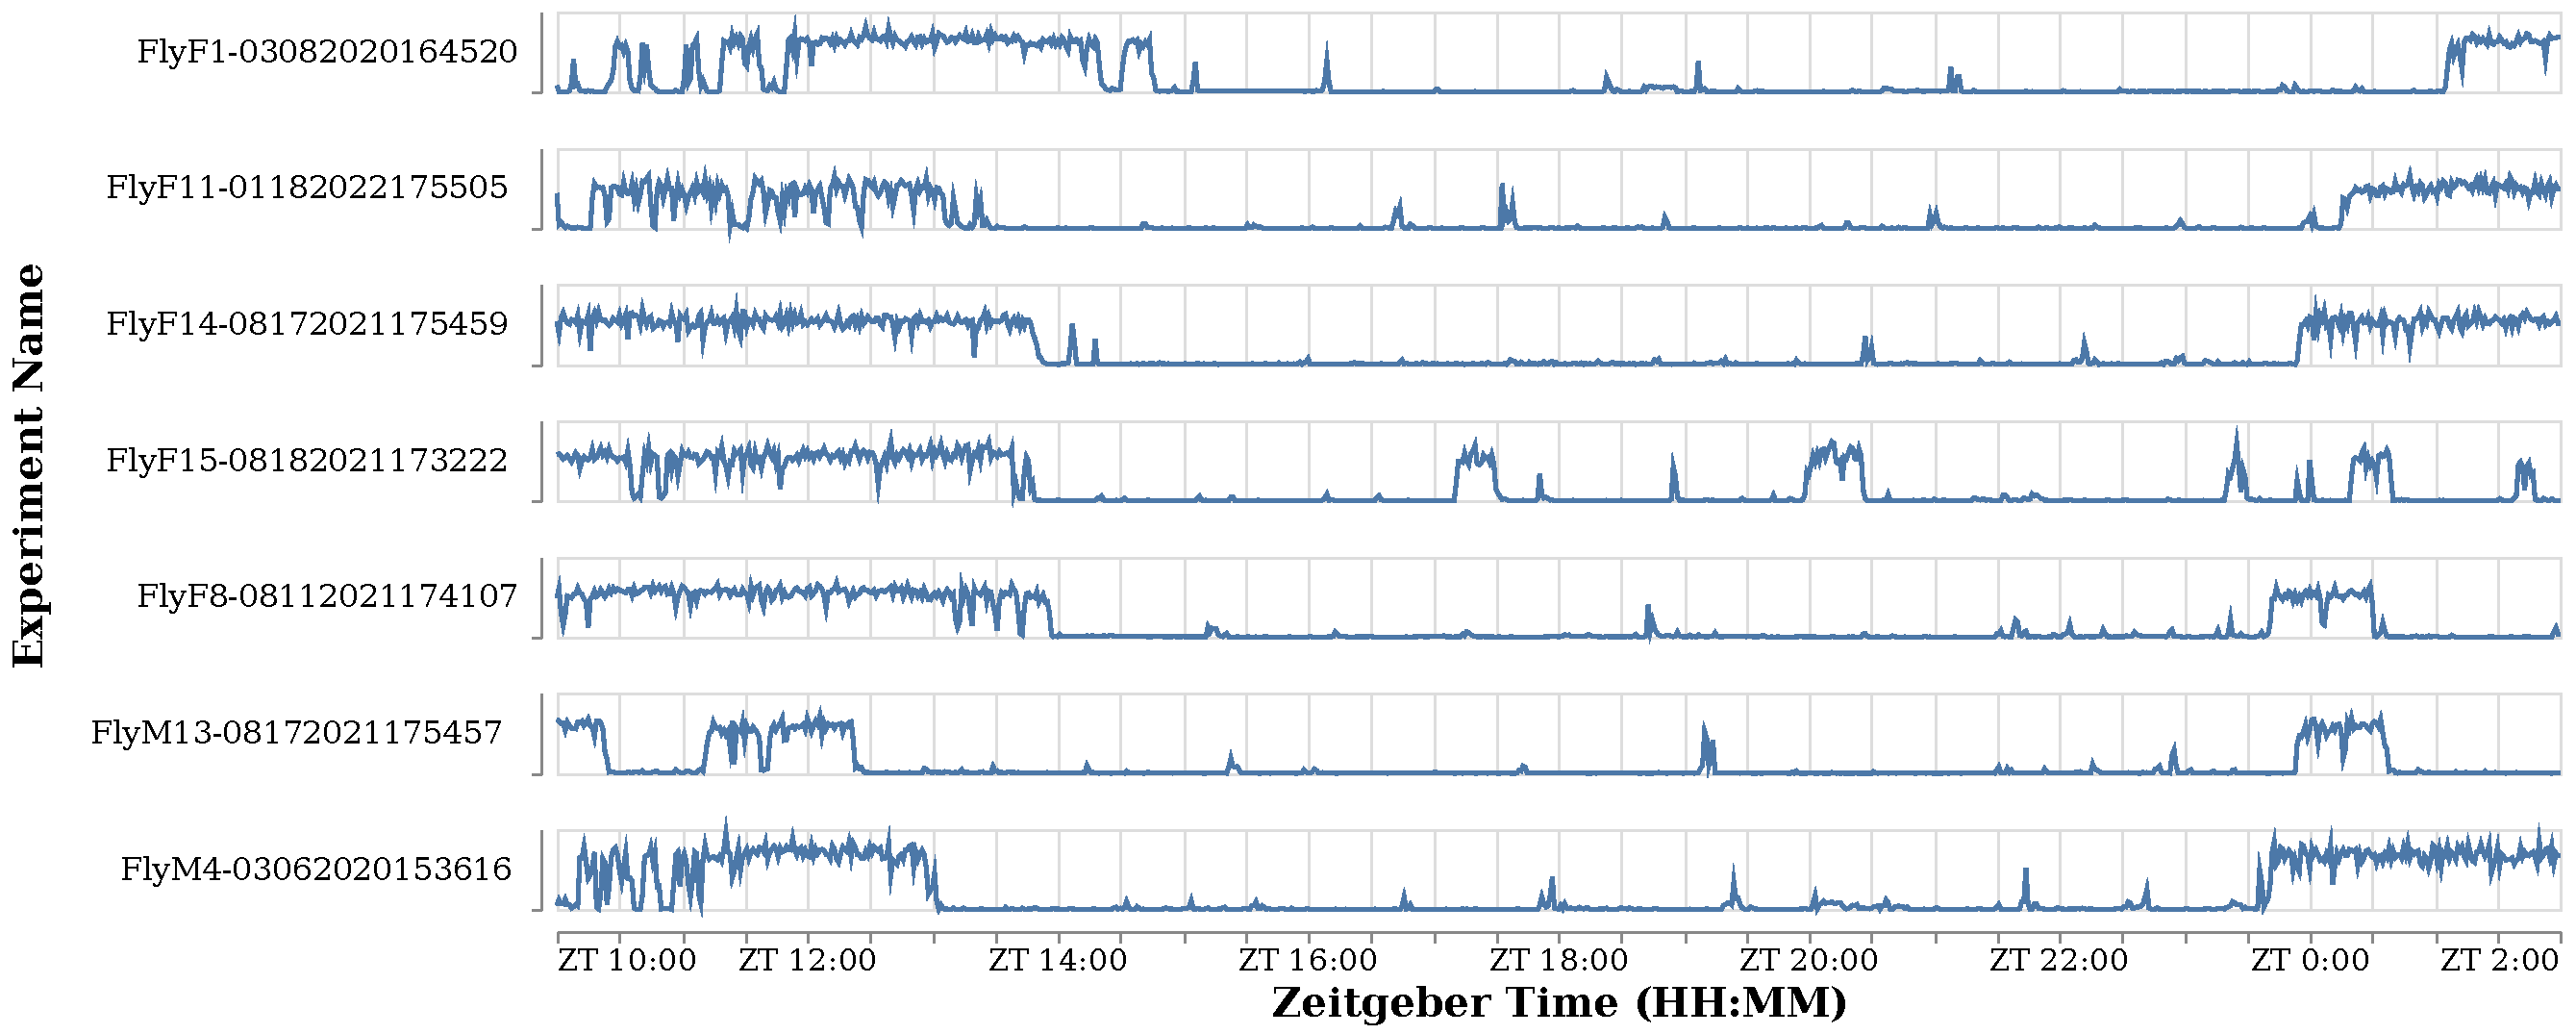
\includegraphics[width=\linewidth]{figures/Velocity-WT-1T.pdf}
		\caption{}
	\end{subfigure}%

	\begin{subfigure}[ht!]{0.85\linewidth}
		\centering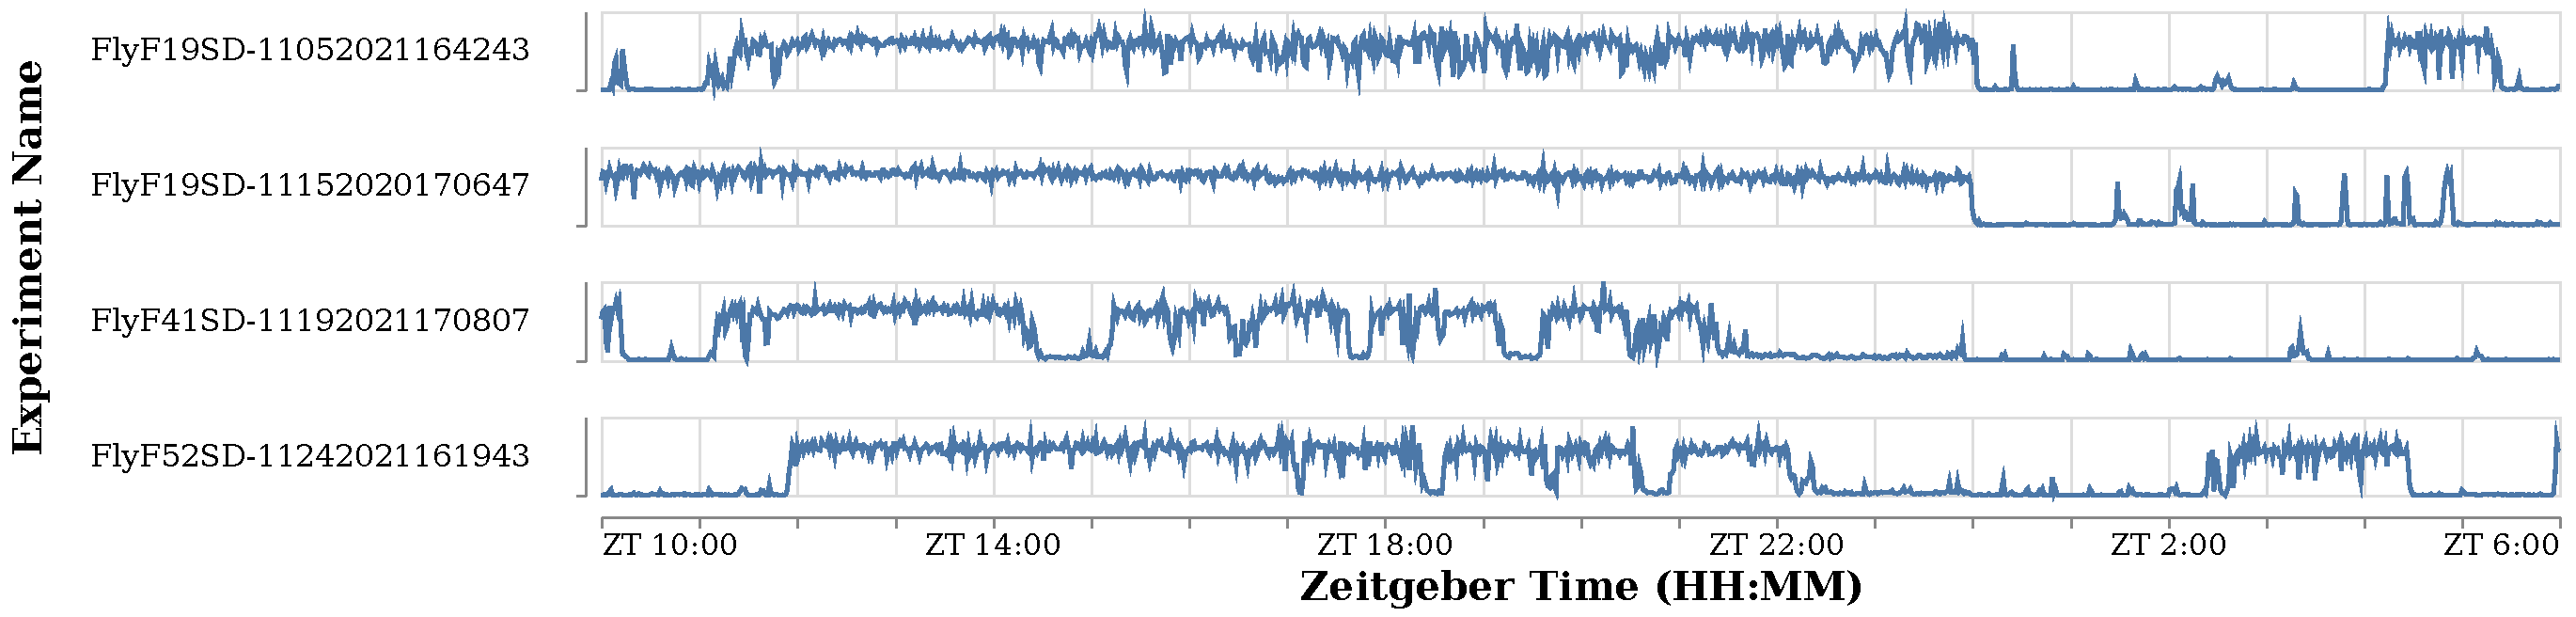
\includegraphics[width=\linewidth]{figures/Velocity-SD-1T.pdf}
		\caption{}
	\end{subfigure}%
\end{figure}

\begin{figure}[ht!]
	\centering
	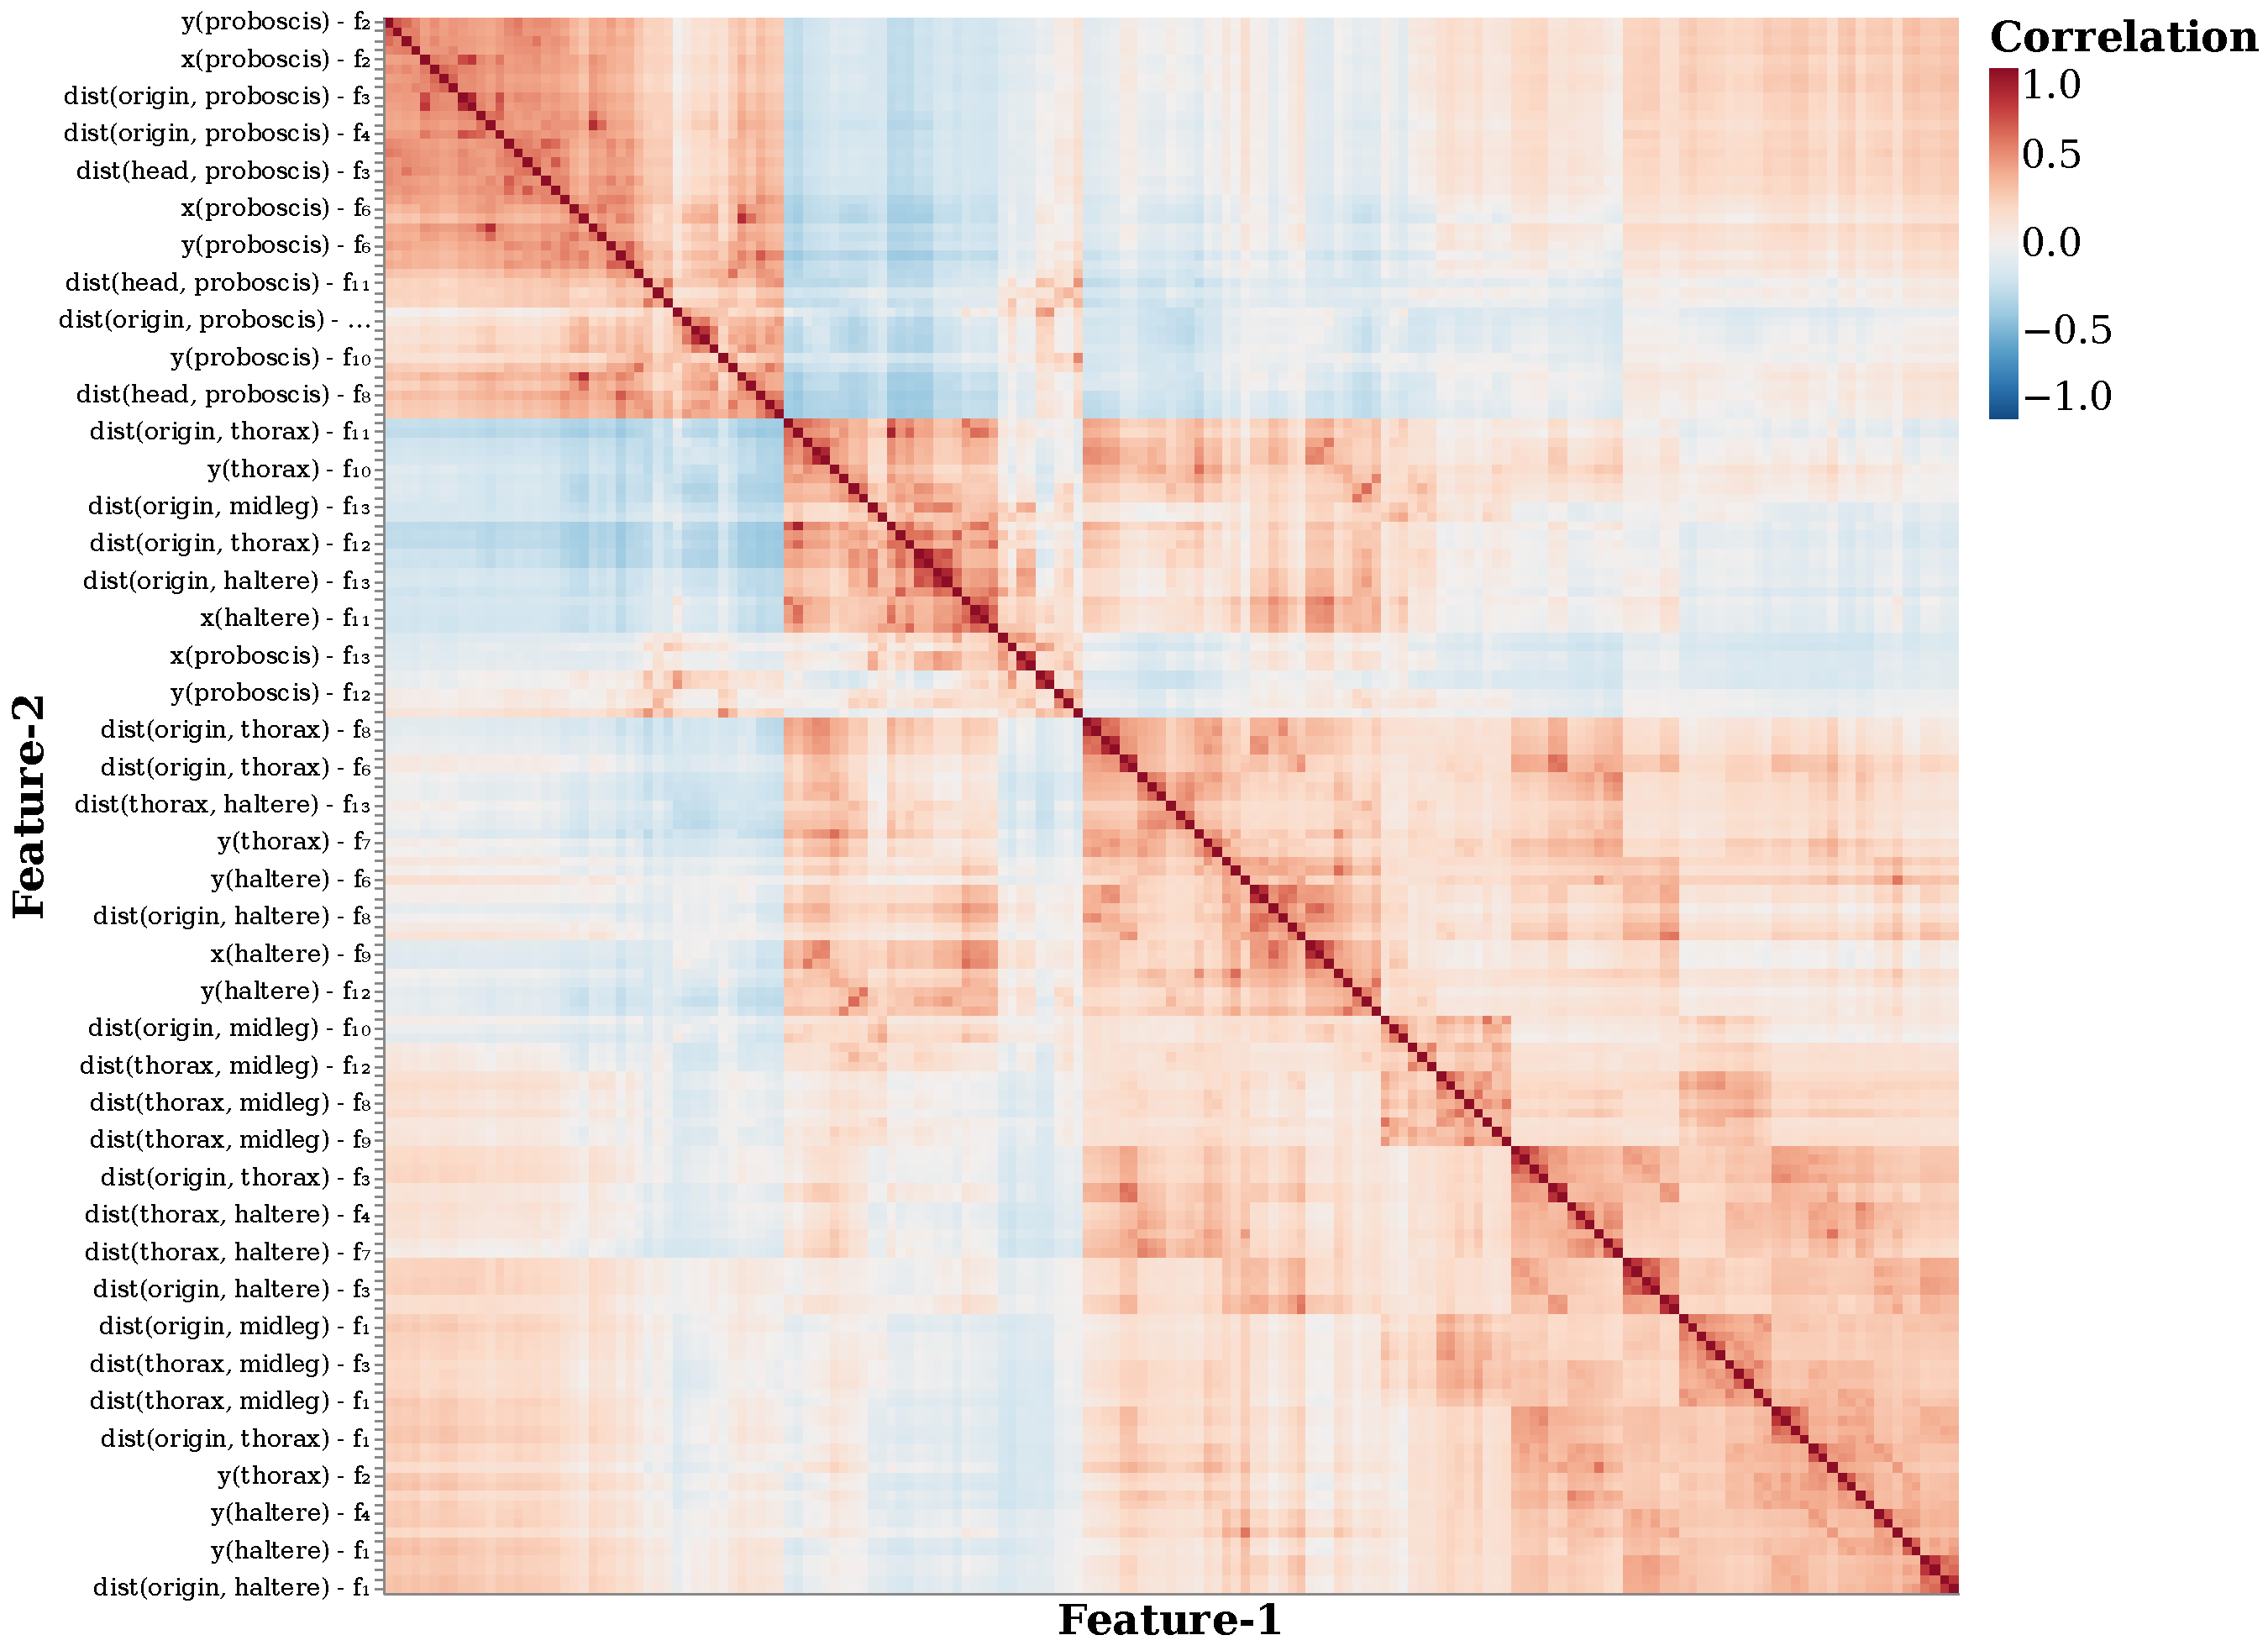
\includegraphics[width=0.70\linewidth]{figures/FeatureCorrelations-FlyF1DAnn.pdf}
	\caption{\label{figure:correlations-btw-features}}
\end{figure}

\begin{figure}[ht!]
	\centering
	\begin{subfigure}[ht!]{0.24\linewidth}
		\centering\includegraphics[width=\linewidth]{example-image-a}
		\caption{\label{figure:supervised-disparate-zoomin-annotations}}
	\end{subfigure}%
	\hfill
	\centering
	\begin{subfigure}[ht!]{0.24\linewidth}
		\centering\includegraphics[width=\linewidth]{example-image-a}
		\caption{\label{figure:unsupervised-disparate-behavioral-regions}}
	\end{subfigure}%
\end{figure}

\begin{figure}[ht!]
	\centering
	\begin{subfigure}[ht!]{0.24\linewidth}
		\centering\includegraphics[width=\linewidth]{example-image-a}
		\caption{}
	\end{subfigure}%
	\hfill
	\centering
	\begin{subfigure}[ht!]{0.24\linewidth}
		\centering\includegraphics[width=\linewidth]{example-image-a}
		\caption{}
	\end{subfigure}%
	\caption{\label{figure:joint-behavioral-embeddings}}
\end{figure}
